\documentclass[12pt,openany]{report}

\usepackage{amsmath,amssymb,amsfonts} %In case we need math stuff
\usepackage{graphicx} %For inserting images and stuff
\usepackage{listings} %For inserting code snippets
\usepackage{enumerate} %For fancy enumeration
\usepackage{hyperref}
\usepackage{color}
\usepackage[margin=2cm]{geometry} %Nice margin setting

\definecolor{dgrey}{rgb}{0.3,0.3,0.3}
\definecolor{dyellow}{rgb}{0.6,0.6,0.1}
\hypersetup{
	colorlinks=true,
	linktoc=all,
	linkcolor=dgrey,
	citecolor=dyellow,
}

\title{ECSE 321 - Intro to Software Engineering\\Deliverable 1}
\author{Harley Wiltzer\\Camilo Garcia La Rotta\\Jake Shnaidman\\Robert Attard\\Matthew Lesko}
\date{February 12, 2017}

\begin{document}
\pagenumbering{gobble} %No page number on title page
\maketitle
\newpage
\pagenumbering{arabic} %Arabic numeral page numbers on regular pages
\tableofcontents
\chapter{Requirements Document}
\section{Functional Requirements}
\textbf{Please Note:}
\begin{itemize}
    \item The requirement's ID is its list number, i.e. 1.1.1.
    \item The priority of requirements starts with the General Requirements from 1.1.1 to 1.1.6, followed by the Non-functional Requirements. 
    More specifically:
        \begin{enumerate}
            \item Total completion of Desktop app requirements in numerical order.
            \item Total completion of Web app in requirements numerical order.
            \item Total completion of Mobile app in requirements numerical order.
            \item Implementation of XML persistence across all platforms.
            \item Implementation of database persistence across all platforms.
            \item Intercommunication between all platforms under a centralized persistence system.
            \item Total completion of Non-functional Requirements in requirements numerical order.
        \end{enumerate} 
\end{itemize}
\subsection{General Requirements}
\begin{enumerate}[\thesubsection .1]
	\item The Teaching Assistant Management System shall include a desktop application.
	\item The Teaching Assistant Management System shall include a web application.
	\item The Teaching Assistant Management System include a mobile application.
	\item All applications (desktop, web, and mobile) shall have an XML persistence layer.
	\item All applications (desktop, web, and mobile) shall have database persistence.
	\item The three applications (desktop, web, and mobile) may be capable of communicating with
		one another.
\end{enumerate}

\subsection{Desktop Application Requirements}
\begin{enumerate}[\thesubsection .1]
	\item The desktop application shall only allow be accessible to users with administrator credentials.
	\item The desktop application shall be written in Java with the Java Swing library.
	\item The desktop application shall be capable of storing in its persistence layer a list of courses with their hours and credits.
	\item The desktop application shall be capable of manipulating a list of courses with their hours and credits from its persistence layer.
	\item The desktop application shall provide the ability to store a list of courses and their attributes listed in (1.2.3).
	\item The desktop application shall be capable of storing the student enrollment data in its persistence layer.
    \item  The desktop application shall be capable of storing the TA/Grader salaries of all McGill Departments from a CSV file onto its persistence layer.
	\item The application shall be capable of accessing TA/Grader schedules from its persistence layer.
	\item The scheduling algorithm shall never appoint work hours for prospective students that are beyond the students' available hours.
	\item The scheduling algorithm shall hire a certain TA for as many time-slots as possible for a given class with multiple lab or tutorial sessions.
	\item The scheduling algorithm shall limit individual TA/Grader hours to within the range of  a minimum of 45 for each course to 180 hours total per semester for all courses.
	\item The scheduling algorithm shall prefer graduate students to undergraduate students.
	\item The scheduling algorithm shall account for students' indicated priorities when assigning job placements.
	\item The desktop application shall provide administrators with the opportunity to review instructor modifications to the TA/Grader hours.
	\item The desktop application shall provide administrators with the opportunity to accept or reject the instructors' modifications.
	\item The desktop application shall be capable of sending job offers to the selected TA's and Graders \textit{once the administrator has explicitly accepted the placements}.
	\item The desktop application shall allow the user to perform the instructor actions described in section 1.2.
	\item The desktop application shall allow the user to perform the TA/Grader actions described in section 1.3.
\end{enumerate}

\subsection{Web Application Requirements}
\begin{enumerate}[\thesubsection .1]
	\item The web application shall only allow be accessible to users with instructor credentials.
	\item The web application shall be programmed in PHP with the use of HTML and CSS.
	\item The web application shall be capable of retrieving the course data from its persistence layer.
	\item The web application shall be capable of displaying the course data from its persistence layer.
	\item The web application shall be capable of retrieving the student enrollment data from its persistence layer.
	\item The web application shall be capable of displaying the student enrollment data from its persistence layer.
	\item The web application shall be capable of creating job postings with the attributes requisite skills and previous experience.
	\item The web application shall be able to save job postings in the persistence layer.
	\item The web application shall be capable of retrieving the course data from its persistence layer.
	\item The application shall be capable of displaying the list of TA/Grader placements from its persistence layer.
	\item The application shall allow the modification of TA/Grader placements without allowing the modifications to cause budget issues.
\end{enumerate}

\subsection{Mobile Application Requirements}
\begin{enumerate}[\thesubsection .1]
	\item The mobile application shall only allow be accessible to users with student credentials.
	\item The mobile application shall be programmed in Java for the Android operating system.
	\item The mobile application shall be created using only the tools provided in the Android UI library in Android Studio.
	\item The mobile application shall be able to create a profile that contains the users' student ID.
	\item The mobile application shall be capable of retrieving a list of job postings from its persistence layer.
	\item The mobile application shall be capable of displaying a list of job postings from its persistence layer.
	\item The mobile application shall limit the amount of applications of the user to a maximum of three.
	\item The mobile application shall allow the arbitrary ranking of job applications by the user.
	\item The mobile application shall be capable of retrieving a list of job offers from its persistence layer.
	\item The mobile application shall be capable of displaying a list of job offers from its persistence layer.
	\item The mobile application shall be capable of submitting acceptance or denial of the aforementioned job offers.
\end{enumerate}

\section{Non-functional Requirements}
\subsection{Performance Requirements}
\begin{enumerate}[\thesubsection .1]
	\item The three applications provided with the product (desktop, web, mobile) shall limit RAM usage to within 750MB.
	\item The scheduling algorithm of the desktop application shall not take longer than one minute to complete.
	\item The three applications shall provide error messages to handle unexpected behavior.
	\item The three applications shall, in case of a system crash, restart the application with the last saved persistence file.
\end{enumerate}

\subsection{Security Requirements}
\begin{enumerate}[\thesubsection .1]
	\item The desktop application shall include a secure authentication procedure to ensure that only administrators gain access.
	\item The web application shall include a secure authentication procedure to ensure that only instructors gain access.
	\item The web application shall be able to identify the current user and associate users with their modification histories.
	\item The mobile application shall include a secure authentication procedure to identify which student is currently using the software. 
	\item The mobile application shall be capable of associating student security information with the respective student account information.
	\item The persistence of administrator, instructor, and student passwords shall be achieved cryptographically, using RSA/NTRU cryptosystems.
\end{enumerate}

\subsection{Compatibility Requirements}
\begin{enumerate}[\thesubsection .1]
	\item The desktop application shall work on Windows 10, Macintosh OS X 10.5 Leopard., GNU/Linux 4.9.8, and BSD 10.3 systems.
	\item The web application shall be compatible with Google Chrome version 25, Mozilla Firefox version 50.0.0, Safari 10, Microsoft Edge, and Internet Explorer 9.
	\item The mobile application shall be compatible with Android phones running Android 4.0 (Ice Cream Sandwich) or a more recent version.
\end{enumerate}
\subsection{Graphical Requirements}
\begin{enumerate}[\thesubsection .1]
	\item The three applications provided with the product (desktop, web, mobile) shall share a common logo (app icon, desktop shortcut, web logo).
	\item The three applications shall have consistent (i.e. the same) color palettes.
	\item The three applications shall have the ability to select between Light and Dark themes for optimal comfort in a variety of lighting conditions.
	\item The color palettes (light theme and dark theme) shall be designed in a color-blind-friendly manner, to promote a common experience to all users. %for Harley's and stuff%
\end{enumerate}
\chapter{TAMAS Domain Model}
The following UMPLE code was written for the generation of the TAMAS domain model:
%\begin{figure}
\lstinputlisting[language=Java,frame=single]{model/TAMAS.ump}
%\end{figure}
%\\
The corresponding class diagram generated by UMPLE may be found below:\\\\
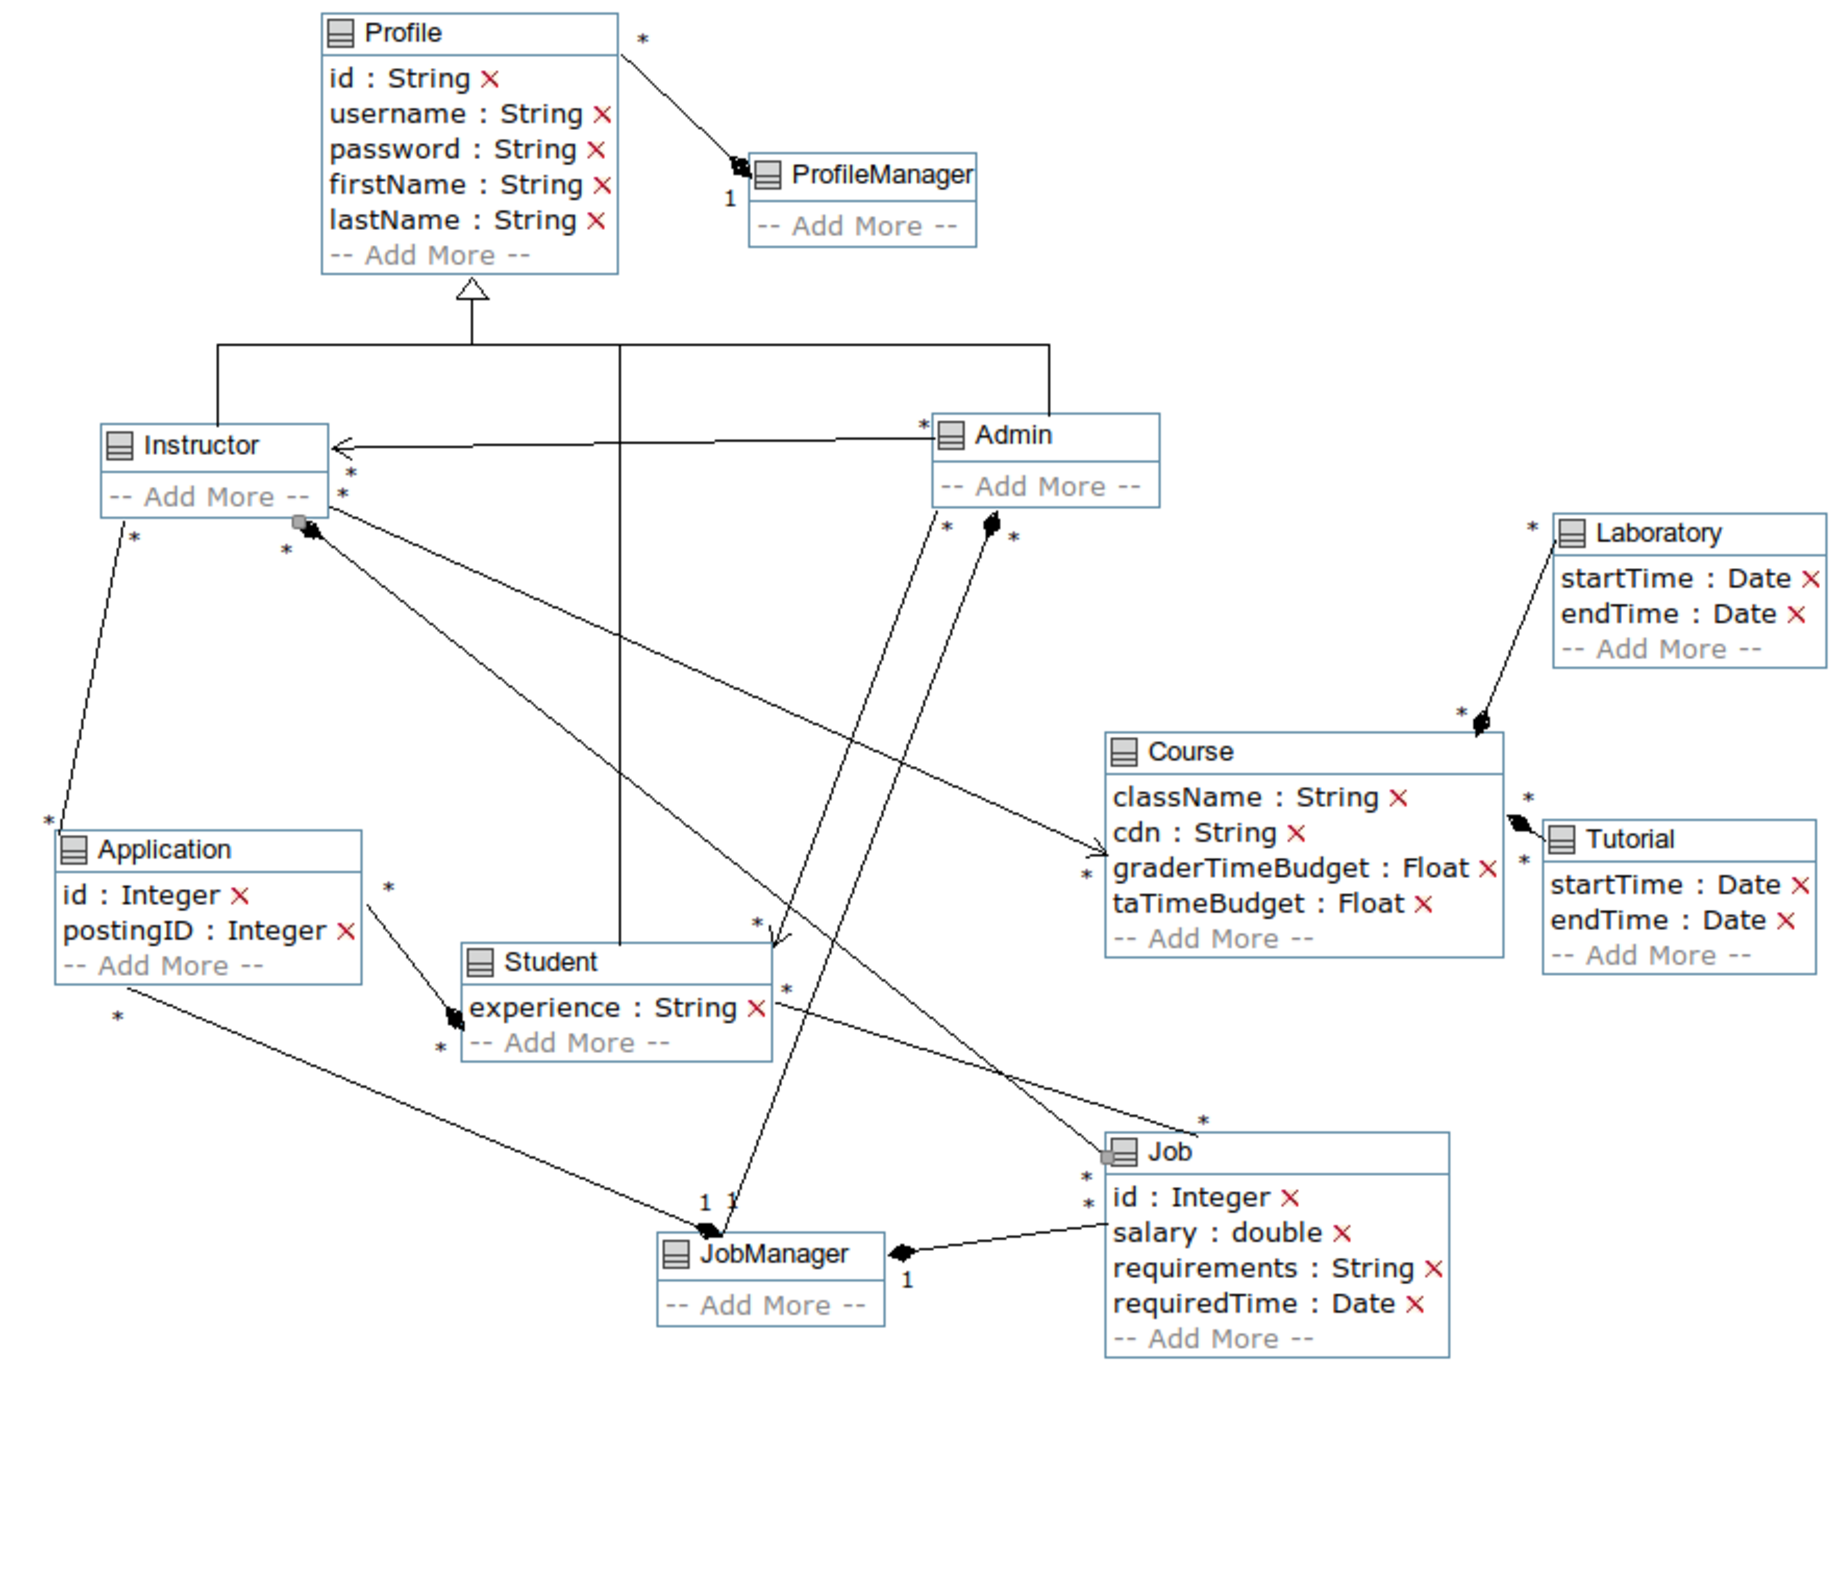
\includegraphics[scale=0.6]{model/Diagrams/classdiagram}

\chapter{Use Cases}
After designing an original use case diagram consisting of all actors and use cases, it was decided
that the diagram was too crowded and thus hard to read. Therefore, three separate use case diagrams
were created in order to alleviate eye strain and clarify the actions. The UML code that was used to
generate the use case diagrams may be found in \hyperref[appA]{Appendix A}.
\section{Use Case Diagrams}
\subsection{Administrator Use Case Diagram}
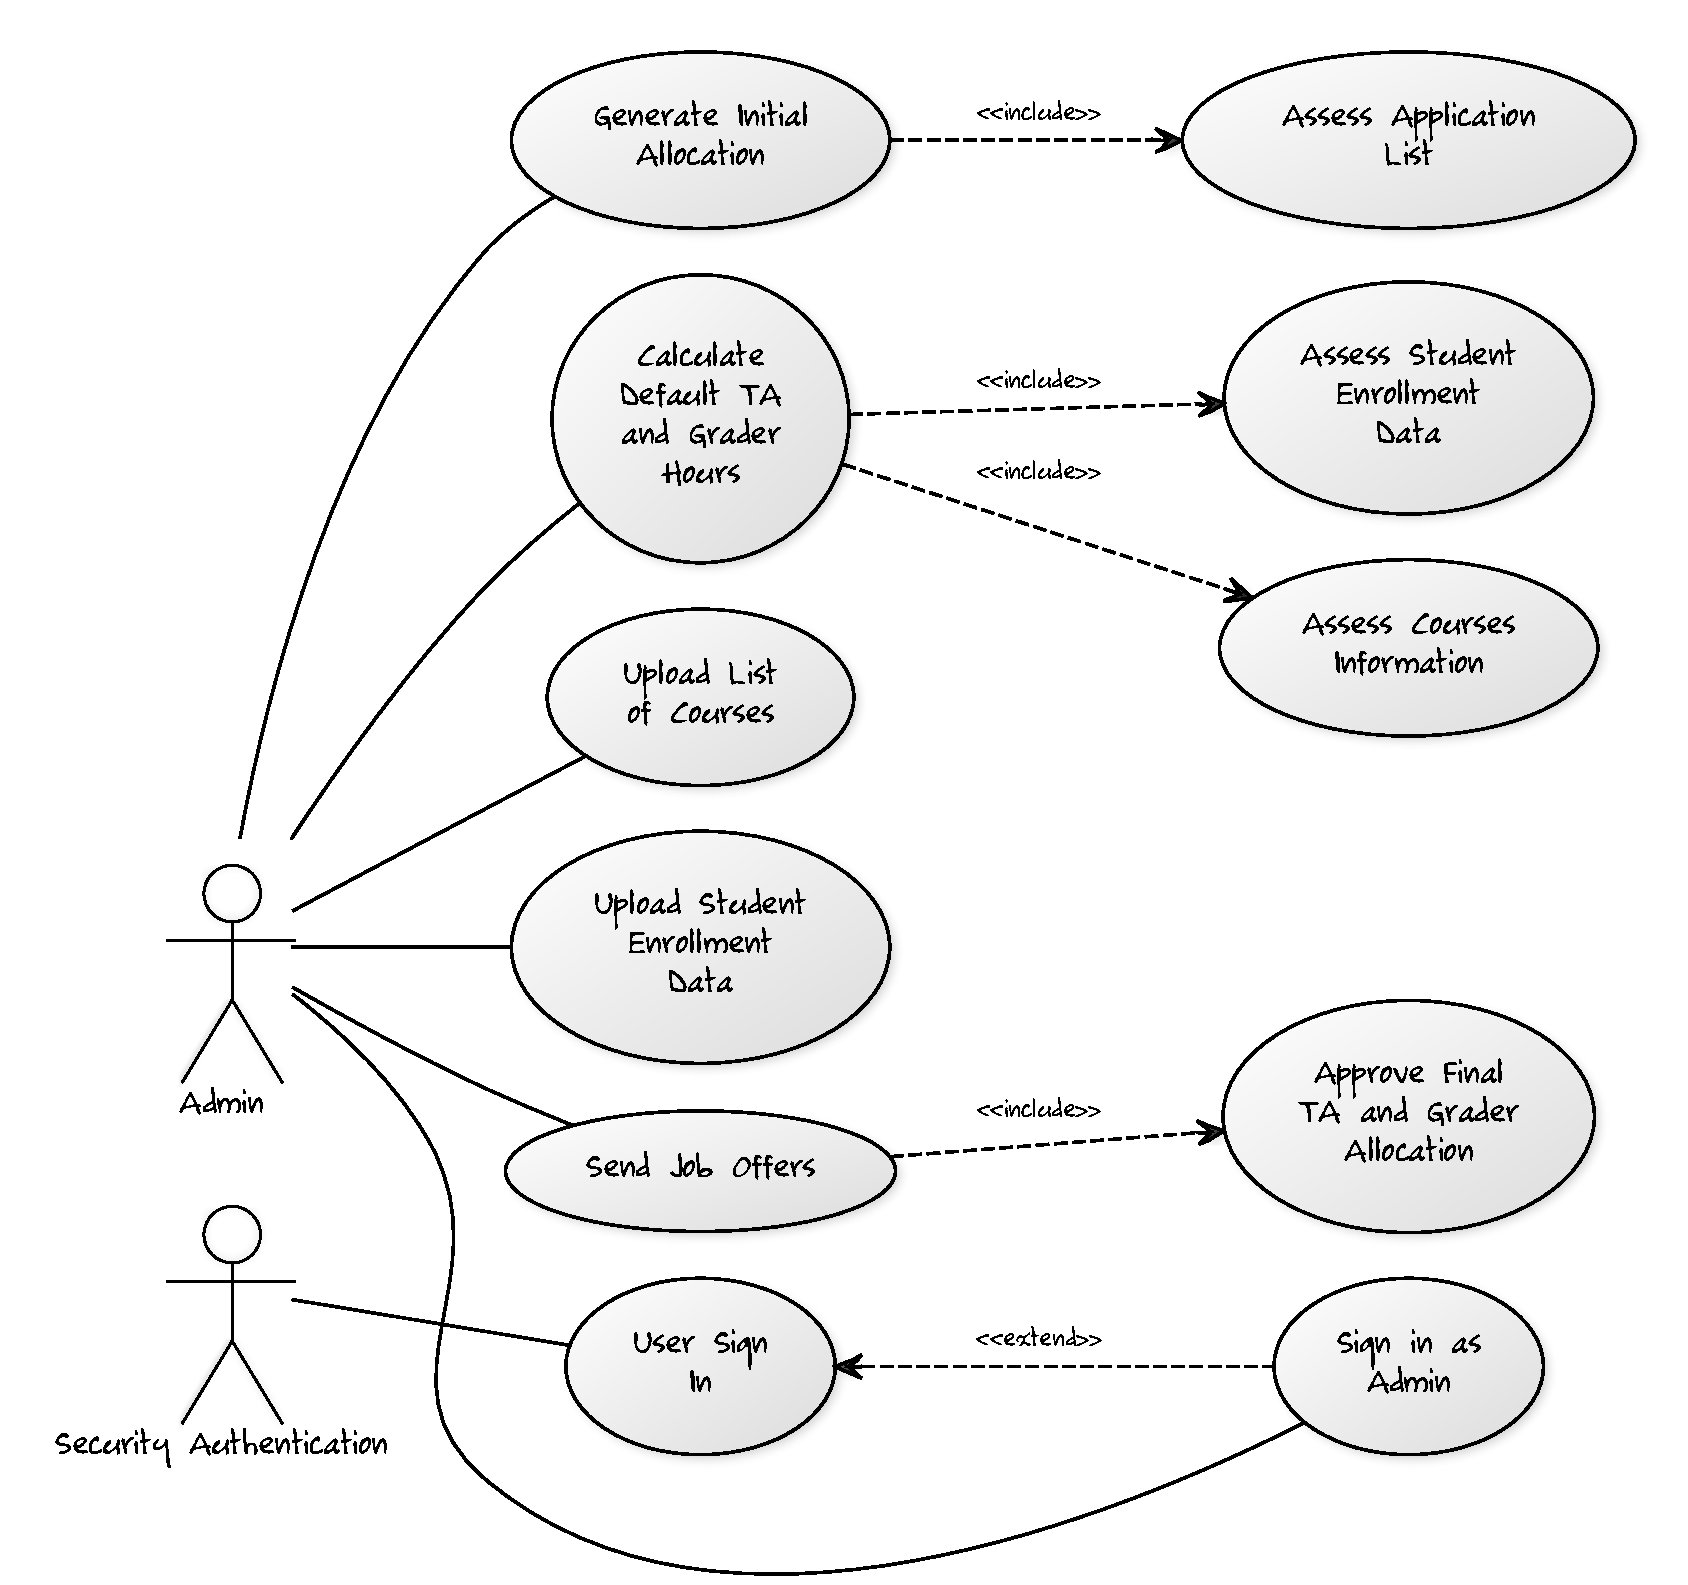
\includegraphics[scale=0.45]{model/Diagrams/UC/adminUC}
\\
Firstly, the \textbf{Administrators} must be able to access the \textit{user sign in form}. This is
extended as \textit{Sign in as Admin} in the use case diagram which is handled by the
\textbf{Security Authentication} actor. The \textbf{administrators} may then \textit{Upload Student
Enrollment Data} and \textit{Upload List of Courses} which contains the information needed to
generate the intitial schedules and budgets needed. \textit{Generate Initial Allocation} includes
\textit{Assess Application List} which takes into account the fact that initial allocation will need
to be assessed by the department. \textit{Calculate Default TA and Grader Hours} include
\textit{Assess Student Enrollment Data} and \textit{Assess Courses Information} which are necessary
to calculate the TA and Grader work hours.
\subsection{Instructor Use Case Diagram}
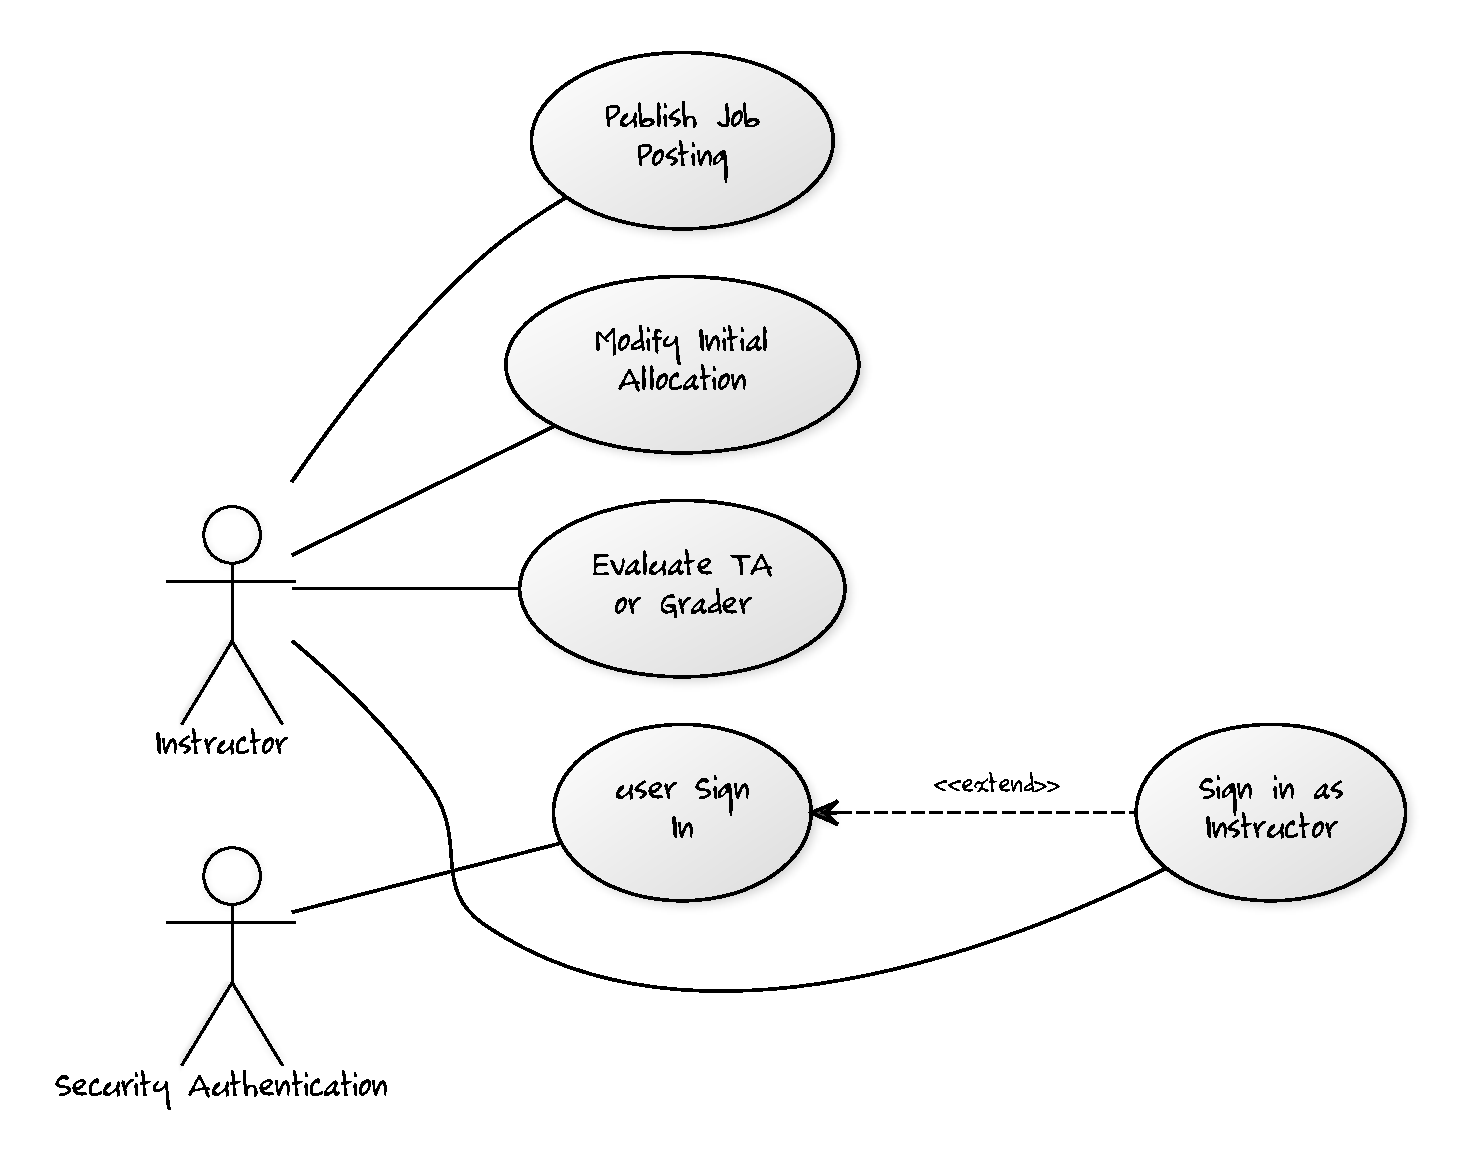
\includegraphics[scale=0.5]{model/Diagrams/UC/instructorUC}
\\
\textbf{Instructors} must be able to access \textit{user sign in} as instructors. \textit{User sign in}
therefore extends \textit{sign in as instructor} which is handled by \textbf{Security
Authentication}. \textbf{Instructors} may then access the \textit{Publish Job Posting} form. After
the job has been published and \textbf{students} have applied, \textbf{instructors} may modify the
first allocation under the \textit{modify initial allocation} use case as needed. After the
semester, the \textbf{instructor} has the ability to access the \textit{Evaluate TA or Grader} form
to provide feedback on the performance of hired \textbf{students}.
\subsection{Student Use Case Diagram}
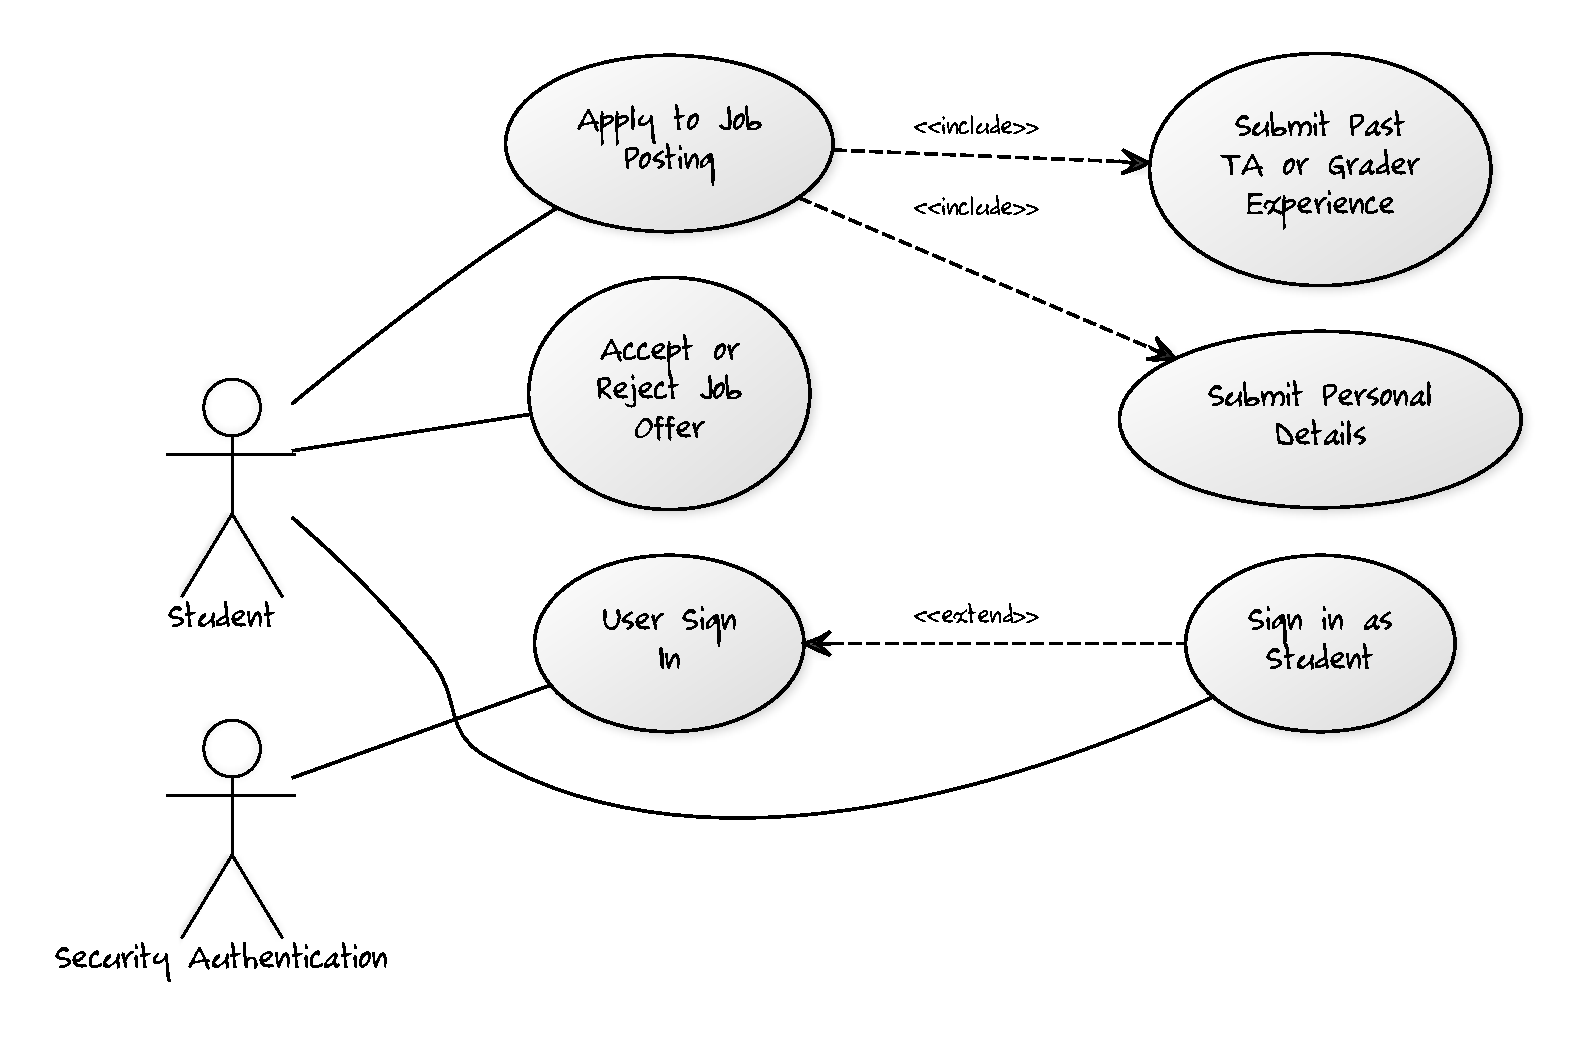
\includegraphics[scale=0.5]{model/Diagrams/UC/studentUC}
\\
\textbf{Students} must be able to access the \textit{user sign in} form as students.
\textbf{Security Authentication} authorizes the \textbf{student} to \textit{sign in as student}.
From there, the \textbf{student} may use the \textit{Apply to Job Posting} forms to apply to
available positions. This includes the use of forms to \textit{Submit Past TA or Grader Experience}
and \textit{Submit Personal Details}. Finally, if job offers are sent to a \textbf{student}, he or
she may access an \textit{Accept or Reject Job Offer} form.
\chapter{Sequence Diagrams}
The following sequence diagrams were designed to display the sequence of actions that will occur in
the use of the applications. One sequence diagram was designed per actor, and another was designed
to demonstrate the authentication process. It is important to note that before authentication, the
user has no identity, and is thus neither a student, an instructor, or an administrator, but just a
default Profile.

\section{Administrator Sequence}
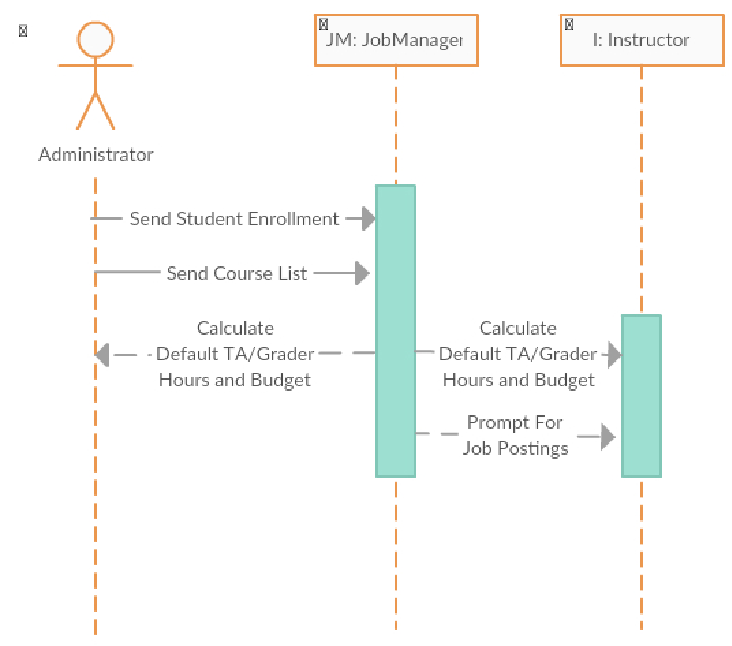
\includegraphics[scale=1.0]{model/Diagrams/Sequence/SeqAdmin}
\section{Instructor Sequence}
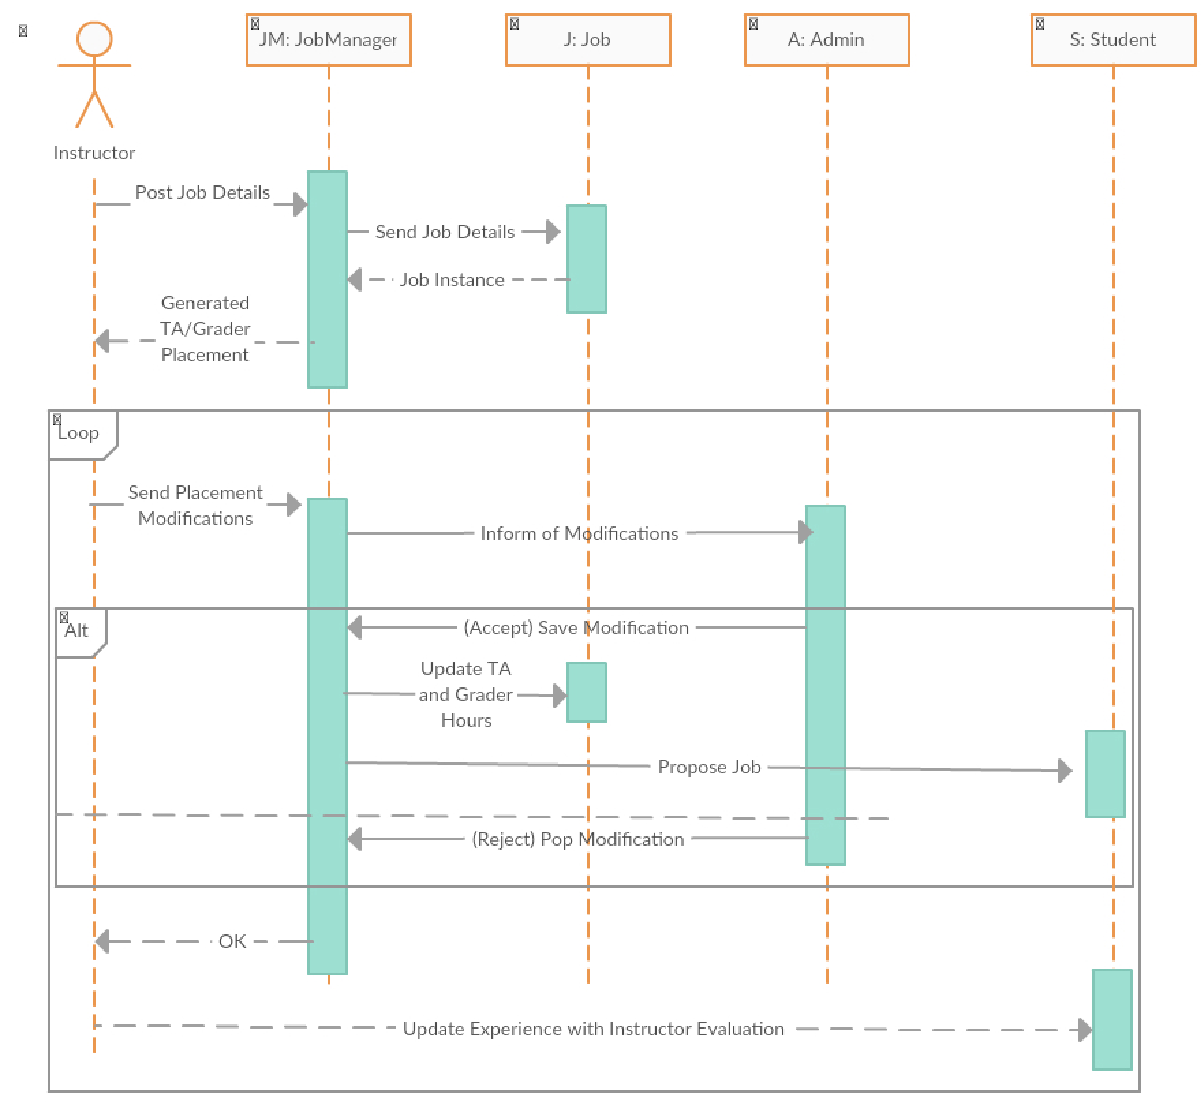
\includegraphics[scale=0.9]{model/Diagrams/Sequence/SeqInstructor}
\section{Student Sequence}
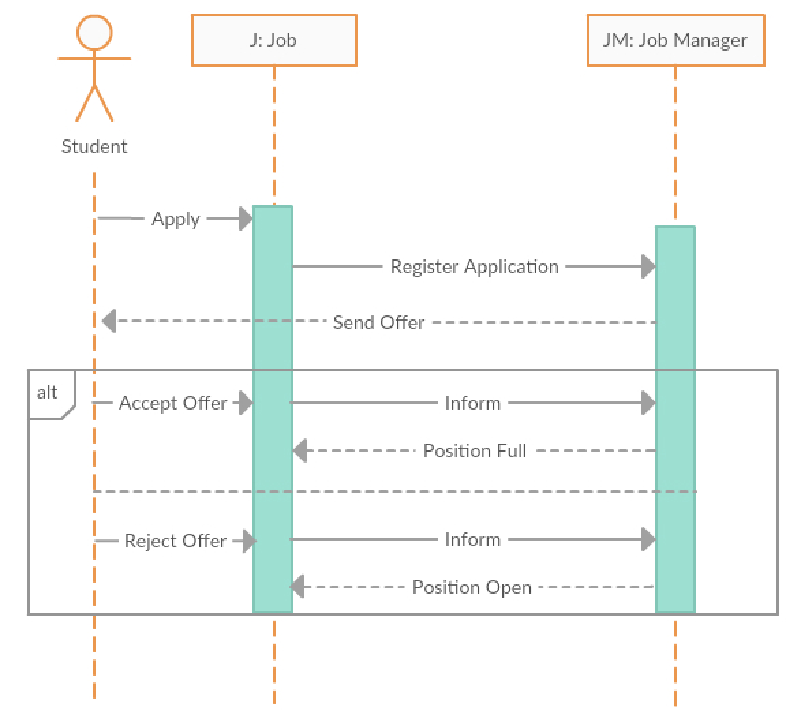
\includegraphics[scale=1.0]{model/Diagrams/Sequence/SeqStudent}
\section{Authentication Sequence}
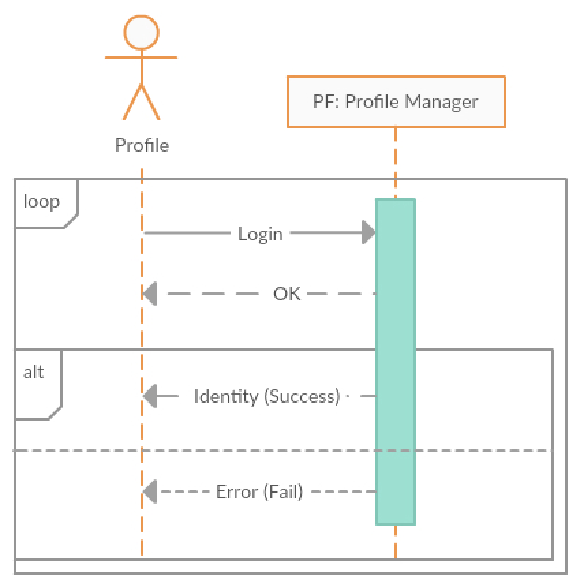
\includegraphics[scale=0.8]{model/Diagrams/Sequence/SeqAuthentication}

\chapter{Statechart for Job Class}
The following statechart was conceived to emphasize the roles and navigations of different states of
the applications. The UML code used to generate the statechart diagram may be seen in
\hyperref[appB]{Appendix B}.\\
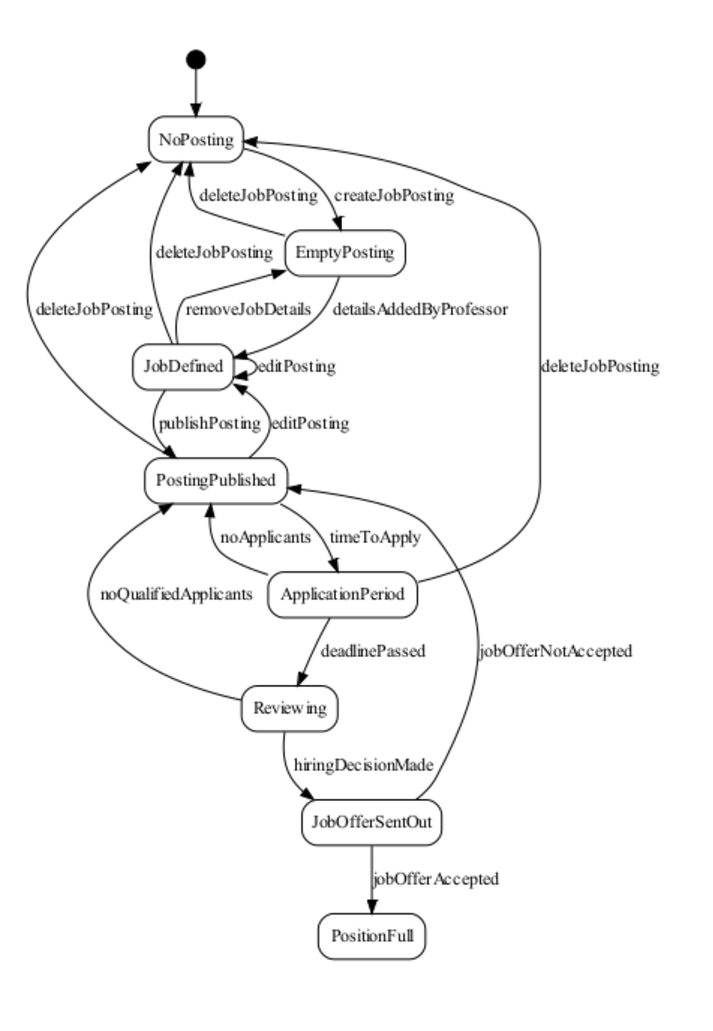
\includegraphics[scale=0.9]{model/Diagrams/StateDiagram/StateChartDiagram.pdf}

\chapter{Work Plan for Remaining Iterations}
%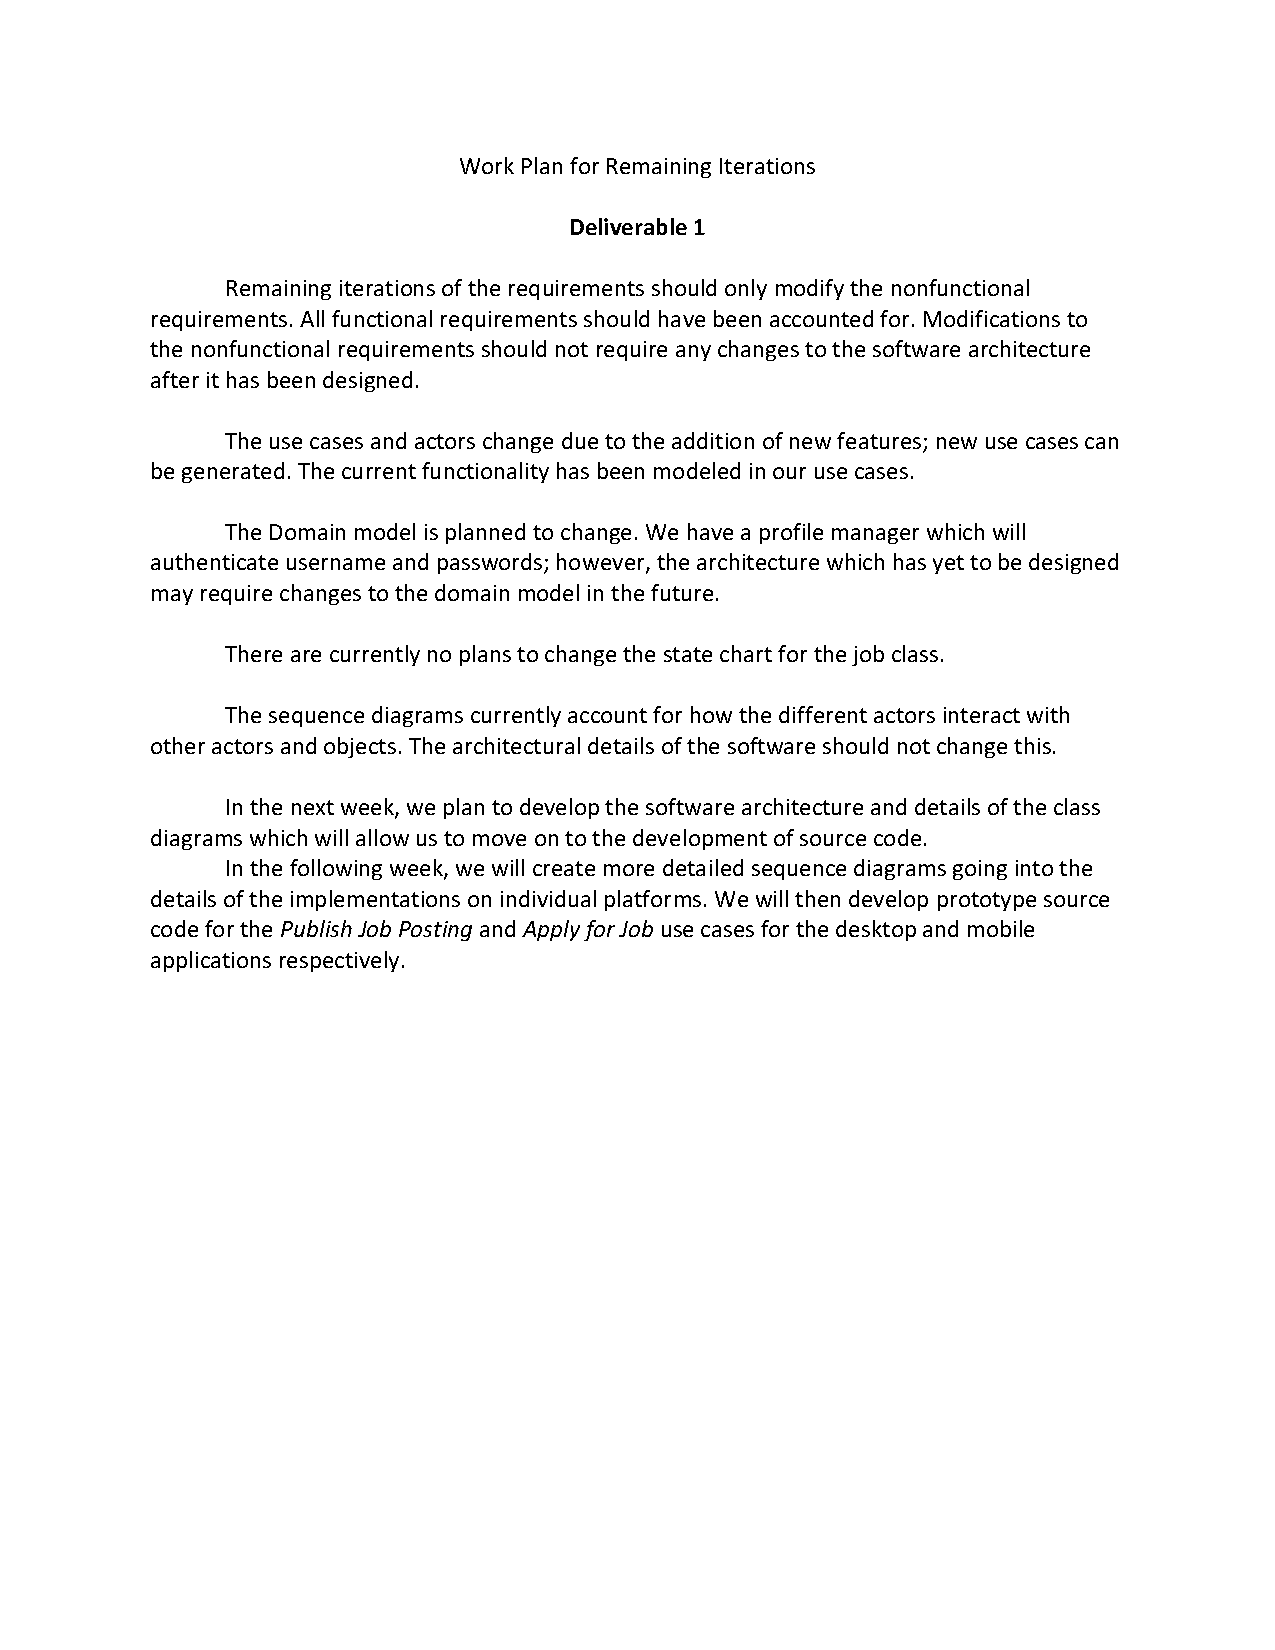
\includegraphics{workplan}
Remaining iterations of the requirements should only modify the nonfunctional
requirements. All functional requirements should have been accounted for. Modifications to
the nonfunctional requirements should not require any changes to the software architecture
after it has been designed.
The use cases and actors change due to the addition of new features; new use cases can
be generated. The current functionality has been modeled in our use cases.
The Domain model is planned to change. We have a profile manager which will
authenticate username and passwords; however, the architecture which has yet to be designed
may require changes to the domain model in the future.
There are currently no plans to change the state chart for the job class.
The sequence diagrams currently account for how the different actors interact with
other actors and objects. The architectural details of the software should not change this.
In the next week, we plan to develop the software architecture and details of the class
diagrams which will allow us to move on to the development of source code.
In the following week, we will create more detailed sequence diagrams going into the
details of the implementations on individual platforms. We will then develop prototype source
code for the \textit{Publish Job Posting} and \textit{Apply for Job} use cases for the desktop and mobile
applications respectively.
\chapter*{Appendix A - Use Case Diagram UML Code}
\label{appA}
\addcontentsline{toc}{chapter}{Appendix A - UML Code for Use Case Diagrams}
\section*{Administrator Use Case}
\lstinputlisting[language=Java,frame=single,breaklines=true]{model/Diagrams/UC/adminUC.txt}
\section*{Instructor Use Case}
\lstinputlisting[language=Java,frame=single,breaklines=true]{model/Diagrams/UC/instructorUC.txt}
\section*{Student Use Case}
\lstinputlisting[language=Java,frame=single,breaklines=true]{model/Diagrams/UC/studentUC.txt}
\chapter*{Appendix B - Statechart UML Code}
\label{appB}
\addcontentsline{toc}{chapter}{Appendix B - UML Code for Statechart}
\lstinputlisting[language=Java,frame=single,breaklines=true]{model/Diagrams/StateDiagram/StateChartUMLCode.ump}
\chapter*{Appendix C - Current Backlog}
\addcontentsline{toc}{chapter}{Appendix C - Current Backlog}
\section*{Week 1}
\addcontentsline{toc}{section}{Week 1}

\subsection*{Main Tasks}

%\textbf{ADD HERE ALL THE SHIT YALL DID}

\begin{itemize}
    \item Harley Wiltzer
	\begin{itemize}
		\item Co-formulated the prototype Requirements Document.
		\item Drafted the first Requirements Document.
		\item Designed Sequence Diagrams for Instructor Actions, Student Actions, Admin Actions.
		\item Made small changes to Class Diagram.
	\end{itemize}
    \item Camilo Garcia La Rotta
    \begin{itemize}
        \item Co-formulated the prototype Requirements Document
        \item Designed the prototype Class Diagram
        \item Structured the GitHub file system
    \end{itemize}
    \item Jacob Shnaidman
		\begin{itemize}
			\item Designed Use Case Diagrams
			\item Wrote Use Case Descriptions
			\item Helped with the design of Sequence Diagrams
			\item Wrote the Work Plan
		\end{itemize}
    \item Robert Attard
    \begin{itemize}
        \item Assisted in preliminary design of the use case diagrams
        \item Designed and improved on the state diagram
        \item Made wording and grammatical changes to Requirements Document
    \end{itemize}
    \item Matthew Lesko
    \begin{itemize}
    	\item Designed the prototype Use Case Diagram
    	\item Co-designed Sequence Diagrams
    \end{itemize}
\end{itemize}

\subsection*{Key Decisions}

%\textbf{ADD HERE ALL THE DECISIONS YALL TOOK}

\begin{enumerate}
    \item \textbf{Requirement Document}
    \item \textbf{Use Cases}
    \begin{itemize}
    	\item Included four actors in the diagram, three of which are users and one of which is a service. The three users are: Student, Instructor and Department (has administrator privileges). The service is a Security Authentication.
    	\item Each user in the diagram acts upon multiple use cases respective to their functionalities mentioned in the Requirements and Specifications documents. Each use case describes functionality that its respective actor has.
    \end{itemize}
    \item \textbf{Class Diagram}
    \begin{itemize}
        \item Trying to mimic the architecture of the event registration app, an early choice was to have a JobManager oversee the job transactions between Instructors and Students
        \item Each user, whether it has administrator, instructor or student access rights, is obliged to have profile instance to facilitate identity access management
		\item Later, it was also decided to have a ProfileManager to handle the actors' profiles and
			their authentication.
        \item To enable an administrator to recreate actions available to instructors or student, we give the class administrator the power to create instances of the aforementioned users
    \end{itemize}
    \item \textbf{Sequence Diagram}
		\begin{itemize}
			\item For convenience and concision, it was decided to design sequence diagrams for each
				main user action.
			\item The sequence diagrams may contain actions from multiple user classes to emphasize
				the sequence. For example, in the Instructor sequence diagram, the action of an
				administrator verifying Instructor modifications to the TA/Grader hours is seen.
			\item The current sequence diagrams include Student actions, Instructor actions,
				Administrator actions, and the authentication process.
		\end{itemize}
    \item \textbf{State Chart}
        \begin{itemize}
            \item The state chart tracks the possible states of the job posting between being created and the position being filled.
            \item The chart also indicates the triggers required to transition between job posting states.

        \end{itemize}
\end{enumerate}

\subsection*{Work Plan}

In the following week, we will create more detailed sequence diagrams going into the details of the implementations on individual platforms. We will then develop prototype source code for the Publish Job Posting and Apply for Job use cases for the desktop and mobile applications respectively.

\subsection*{Work Hours}

\begin{itemize}
    \item Harley Wiltzer
		\begin{itemize}
			\item Requirements document: 1 hours
			\item Sequence diagrams: 3 hours
			\item Class diagram: 30 minutes
			\item Compilation of report: 4 hours
		\end{itemize}
    \item Camilo Garcia La Rotta
    \begin{itemize}
        \item Requirements document: 2 hours
        \item Class diagram: 2 hours
        \item State diagram: 1 hour
    \end{itemize}
    \item Jacob Shnaidman
    \begin{itemize}
        \item Use Case Diagrams: 4 hours
        \item Use Case Description 1.5 hours
		\item Helped with Sequence Diagrams 0.5 hours
		\item Work Plan 0.5 hours
    \end{itemize}
    \item Robert Attard
    \begin{itemize}
        \item Requirements document: 0.5 hours
        \item Use Case diagram: 3.5 hours
        \item State diagram: 3 hours
    \end{itemize}
    \item Matthew Lesko
    \begin{itemize}
    	\item Use case diagram: 4 hours
    	\item Co-design sequence diagrams: 4 hours
    \end{itemize}
\end{itemize}
\end{document}
